\chapter{Bài 1. Khái quát về môn vật lí}
\begin{center}
	\textit{(2 tiết)}
\end{center}
\section{MỤC TIÊU DẠY HỌC}
\begin{center}
	\begin{longtable}{|M{2.5cm}|L{12.5cm}|M{2cm}|}
		\hline
		\thead{Biểu hiện\\ năng lực} & \thead{Mục tiêu} & \thead{STT}\\
		\hline
		\multicolumn{3}{|c|}{\textbf{ Năng lực vật lí}}\\
		\hline
		1.1 & Nêu được đối tượng nghiên cứu của Vật lí học và mục tiêu của môn Vật lí.  & 1\\
		\hline
		
		1.2 & Nêu được một số ví dụ về phương pháp nghiên cứu vật lí (phương pháp thực nghiệm và phương pháp lí thuyết). &2\\
		\hline
		2.1 - 2.3 & Mô tả được các bước trong tiến trình tìm hiểu thế giới tự nhiên dưới góc độ vật lí. & 3\\
		\hline
		1.2 & Nêu được ví dụ chứng tỏ kiến thức, kĩ năng vật lí được sử dụng trong một số lĩnh vực khác nhau.& 4\\
		\hline
		3.1 & Phân tích được một số ảnh hưởng của vật lí đối với cuộc sống, đối với sự phát triển của khoa học, công nghệ và kĩ thuật.&5\\
		\hline
		\multicolumn{3}{|c|}{\textbf{Năng lực chung}}\\
		\hline
		TC - TH & Chủ động, tích cực thực hiện những công việc của bản thân trong học tập qua việc tham gia góp ý tưởng, đặt câu hỏi và trả lời các câu thảo luận.	& 6\\
		\hline
		GT - HT & Biết sử dụng ngôn ngữ kết hợp với các loại phương tiện phi ngôn ngữ đa dạng để trình bày thông tin, ý tưởng và thảo luận, lập luận để giải quyết các vấn đề được đặt ra trong bài học. & 7\\
		\hline
	\end{longtable}
\end{center}
\section{THIẾT BỊ DẠY HỌC VÀ HỌC LIỆU}
\begin{itemize}
	\item Tivi/máy chiếu.
	\item Giấy A3/bảng nhóm, thẻ nội dung.
\end{itemize}
\section{TIẾN TRÌNH DẠY HỌC}
\subsection{TIẾN TRÌNH}
\newpage
\begin{center}
	\begin{longtable}{|L{2.75cm}|C{1.25cm}|L{5cm}|L{3.5cm}|L{4cm}|}
		\hline
		\thead{Tiến trình} & \thead{Mục\\tiêu} & \thead{Nội dung dạy học \\trọng tâm} & \thead{PP,\\ KTDH} & \thead{Phương pháp \\đánh giá}\\
		\hline
		\textbf{Hoạt động 1:} Tìm hiểu đối tượng nghiên cứu và mục tiêu của vật lí & 1, 6 & Đối tượng nghiên cứu của vật lí, mục tiêu của vật lí & PP: Đàm thoại & GV đánh giá dựa trên câu trả lời của học sinh.\newline
		PP đánh giá: quan sát, nghe. \\
		\hline
		\textbf{Hoạt động 2:} Tìm hiểu phương pháp nghiên cứu vật lí & 2, 3, 7 & Phương pháp thực nghiệm và phương pháp lí thuyết trong nghiên cứu vật lí, tiến trình tìm hiểu tự nhiên dưới góc độ vật lí  &PP: Dạy học hợp tác \newline KTDH: Đọc tích cực & GV đánh giá dự trên hoạt động thảo luận nhóm và bài báo cáo của nhóm HS.\newline PP đánh giá: quan sát, nghe.\\
		\hline
		\textbf{Hoạt động 3:} Tìm hiểu ảnh hưởng của vật lí trong một số lĩnh vực & 4, 5, 7 & Một số ảnh hưởng của vật lí đối với cuộc sống, đối với sự phát triển của khoa học, công nghệ và kĩ thuật.  &PP: Dạy học hợp tác \newline KTDH: Kĩ thuật "tia chớp" & GV đánh giá dự trên hoạt động thảo luận nhóm và phần tham gia trả lời nhanh của đại diện các nhóm.\newline PP đánh giá: quan sát, nghe.\\
		\hline
		\textbf{Hoạt động 4:} Luyện tập & 1, 2, 3, 4, 5, 6 & Củng cố kiến thức, giải bài tập & PP: Đàm thoại  & GV đánh giá dự trên bài tập cá nhân của học sinh và câu hỏi các em đặt ra để thảo luận.\newline PP đánh giá: quan sát, nghe.\\
		\hline
	\end{longtable}
\end{center}
\subsection{CÁC HOẠT ĐỘNG HỌC}
\hoatdong{Tìm hiểu đối tượng nghiên cứu và mục tiêu của vật lí}
{HS nêu được đối tượng nghiên cứu của Vật lí học và mục tiêu của môn Vật lí.

}
{
Câu trả lời của HS.
}
{
\textit{\underline{* GV chuyển giao nhiệm vụ học tập}}\\
GV giới thiệu về ý nghĩa thuật ngữ "vật lí". \\
GV yêu cầu học sinh suy nghĩ về câu hỏi thảo luận 1: Nêu đối tượng nghiên cứu tương ứng với từng phân ngành của vật lí: cơ, ánh sáng, điện, từ.\\
Từ câu trả lời tổng hợp của các HS. GV rút ra kết luận về đối tượng nghiên cứu và mục tiêu của vật lí.\\
\textit{\underline{* HS thực hiện nhiệm vụ học tập}}\\
HS lắng nghe phần giới thiệu của GV và tham gia trả lời câu hỏi thảo luận 1.
}

\hoatdong{Tìm hiểu phương pháp nghiên cứu vật lí}
{
HS nêu được một số ví dụ về phương pháp nghiên cứu vật lí (phương pháp thực nghiệm và phương pháp lí thuyết).

 HS mô tả được tiến trình tìm hiểu thế giới tự nhiên dưới góc độ vật lí
}
{Phiếu học tập 1.\\
	Sơ đồ tiến trình tìm hiểu thế giới tự nhiên dưới góc độ vật lí.

}
{
	\textit{\underline{
* GV chuyển giao nhiệm vụ học tập	
}}\\
GV chia lớp học thành 4 nhóm.\\
GV yêu cầu các nhóm HS đọc SGK Vật lí 10 CTST mục "Phương pháp nghiên cứu của vật lí" trang 6 - 9, thảo luận theo nhóm và thực hiện 2 nhiệm vụ học tập sau:
\begin{itemize}
	\item Phân biệt phương pháp lí thuyết và phương pháp thực nghiệm trong nghiên cứu vật lí, đưa ra 2 ví dụ cho mỗi phương pháp.
	\item Sơ đồ hoá quá trình tìm hiểu thế giới tự nhiên dưới góc độ vật lí từ các thẻ nội dung được gợi ý trong phiếu học tập 1.
\end{itemize}
GV yêu cầu các nhóm HS thực hiện nhiệm vụ học tập trong 15 phút.\\
\textit{\underline{
* HS thực hiện nhiệm vụ học tập
}}\\
Các nhóm HS tiến hành đọc tích cực, thảo luận và trình bày kết quả thảo luận vào phiếu học tập 1.\\
GV: Theo dõi để phát hiện vấn đề mà các nhóm gặp phải, từ đó đưa ra sự định hướng, hỗ trợ phù hợp cho mỗi nhóm.\\
\textit{\underline{
* HS báo cáo kết quả thực hiện nhiệm vụ học tập}}\\
GV mời đại diện 1 nhóm HS trình bày bảng phân biệt phương pháp lí thuyết và phương pháp thực nghiệm. Các nhóm còn lại theo dõi, góp ý, bổ sung.\\
GV nhận xét, chuẩn hoá kiến thức.\\
GV mời đại diện 4 nhóm HS trình bày lên bảng sơ đồ mô tả tiến trình tìm hiểu thế giới tự nhiên dưới góc độ vật lí.\\
GV cho các nhóm nhận xét chéo.\\
GV chỉnh lí, hợp thức hoá kiến thức.
}
%========================================================
\hoatdong{
Tìm hiểu ảnh hưởng của vật lí trong một số lĩnh vực.
}
{
HS trình bày được một số ảnh hưởng của vật lí đối với cuộc sống, đối với sự phát triển của khoa học, công nghệ và kĩ thuật.
}
{Biên bản thảo luận nhóm và phần trình bày của HS.

}
{
	\textit{\underline{
* GV chuyển giao nhiệm vụ học tập	
}}\\
GV chia mỗi dãy bàn thành 1 nhóm.\\
GV yêu cầu HS làm việc theo nhóm, đọc SGK mục 2: Ảnh hưởng của vật lí đến một số lĩnh vực trong đời sống kĩ thuật kết hợp với kiến thức thực tiễn để liệt kê nhiều nhất \textit{(có thể)} những ứng dụng của vật lí trong các lĩnh vực:
\begin{itemize}
	\item Đời sống hằng ngày.
	\item Thông tin liên lạc.
	\item Y tế.
	\item Công nghiệp.
	\item Nông nghiệp.
	\item Nghiên cứu khoa học.
\end{itemize}
\textit{\underline{
* HS thực hiện nhiệm vụ học tập
}}\\
HS thảo luận theo nhóm được phân công.\\
GV: Theo dõi để phát hiện vấn đề mà các nhóm gặp phải, từ đó đưa ra sự định hướng, hỗ trợ phù hợp cho mỗi nhóm.\\
\textit{\underline{
		* HS báo cáo kết quả thực hiện nhiệm vụ học tập
}}\\
GV sử dụng kĩ thuật "tia chớp" để HS trình bày kết quả thảo luận: GV yêu cầu mỗi nhóm đại diện 2 HS lên bảng xếp thành hàng ngang. GV đưa ra lĩnh vực bất kì, HS lần lượt đưa ra hồi đáp về 1 ảnh hưởng của vật lí đến lĩnh vực đó trong 5 giây, nếu sau 5 giây HS không đưa ra được lời hồi đáp sẽ bị loại. Nhóm nào còn lại HS cuối cùng trên bảng sẽ là nhóm chiến thắng.\\
GV chỉnh lí, hợp thức hoá kiến thức.
}
%=====================================================
\hoatdong{
	Luyện tập.
}
{ HS nhận biết được đối tượng và mục tiêu nghiên cứu vật lí.\\
	HS phân biệt được phương pháp thực nghiệm và phương pháp lí thuyết trong nghiên cứu vật lí.\\
	HS vận dụng được tiến trình tìm hiểu thế giới tự nhiên dưới góc độ vật lí.
}
{
	Bài tập cá nhân của học sinh.
}
{
	\textit{\underline{GV chuyển giao nhiệm vụ học tập}}\\
	GV lần lượt chuyển giao từng bài tập, yêu cầu HS hoạt động cá nhân để giải.\\
	\textit{\underline{HS thực hiện nhiệm vụ học tập}}\\
	HS \textit{(làm việc cá nhân)}:  Giải bài tập trong đề cương. 
	
	GV: Theo dõi để phát hiện các HS gặp khó khăn, từ đó đưa ra sự định hướng, hỗ trợ phù hợp cho mỗi HS.\\
	\textit{\underline{HS báo cáo kết quả thực hiện nhiệm vụ học tập}}\\
	GV: Mời HS lên bảng giải bài tập.
	
	HS: Đặt câu hỏi, góp ý.
	
	GV: Chỉnh lí, hợp thức hoá kiến thức.
}

\section{HỒ SƠ DẠY HỌC}
\subsection{NỘI DUNG DẠY HỌC}
\begin{enumerate}[label=\bfseries\arabic*.]
	\item \textbf{Đối tượng - Mục tiêu - Phương pháp nghiên cứu vật lí}
	\begin{itemize}
		\item Đối tượng: Các dạng vận động của vật chất và năng lượng.
		\item Mục tiêu: Khám phá ra qui luật tổng quát nhất chi phối sự vận động của vật chất và năng lượng, cũng như tương tác giữa chúng ở mọi cấp độ: vĩ mô, vi mô.
		\item Phương pháp nghiên cứu: Phương pháp thực nghiệm và phương pháp lí thuyết.
		\begin{itemize}
			\item Phương pháp thực nghiệm dùng thí nghiệm để phát hiện kết quả mới giúp kiểm chứng, hoàn thiện, bổ sung hay bác bỏ giả thuyết nào đó. Kết quả mới này cần được giải thích bằng lí thuyết đã biết hoặc lí thuyết mới.
			\item Phương pháp lí thuyết sử dụng ngôn ngữ toán học và suy luận lí thuyết để phát hiện một kết quả mới. Kết quả mới này cần được kiểm chứng bằng thực nghiệm.
		\end{itemize}
	Hai phương pháp này hỗ trợ cho nhau, trong đó phương
	pháp thực nghiệm có tính quyết định.
	\item Quá trình nghiên cứu khoa học gồm các bước sau:
	\begin{enumerate}[label=\bfseries Bước \arabic*.]
		\item Quan sát hiện tượng để xác định đối tượng nghiên cứu.
		\item Quan sát hiện tượng để xác định đối tượng nghiên cứu.
		\item Thiết kế, xây dựng mô hình lí thuyết hoặc mô hình thực nghiệm để kiểm chứng giả thuyết.
		\item Tiến hành tính toán theo mô hình lí thuyết hoặc thực hiện thí nghiệm để thu thập dữ liệu. Sau đó xử lý số liệu và phân tích kết quả để xác nhận, điều chỉnh, bổ sung hay loại bỏ mô hình, giả
		thuyết ban đầu.
		\item Rút ra kết luận.
	\end{enumerate}
	\end{itemize}
\item \textbf{Ảnh hưởng của vật lí đến một số lĩnh vực trong đời sống và kĩ thuật}\\
\begin{itemize}
	\item Vật lí ảnh hưởng mạnh mẽ và có tác động làm thay đổi mọi lĩnh vực hoạt động của con người: Thông tin liên lạc - Y tế - Công nghiệp – Nông nghiệp – Nghiên cứu khoa học.
	\item Kiến thức Vật lí trong các phân ngành được áp dụng kết hợp để tạo ra kết quả tối ưu. Các kĩ năng vật lí như tính chính xác, đúng	thời điểm và thời lượng, quan sát, suy luận nhạy bén,\dots đã trở
	thành kĩ năng sống cần có của con người hiện đại.
\end{itemize}
\end{enumerate}

\subsection{CÁC HỒ SƠ KHÁC}
Phiếu học tập
\begin{center}
	\begin{longtable}{|L{8.5cm}|L{8.5cm}|}
		\hline
		\multicolumn{2}{|M{17cm}|}{\thead{PHIẾU HỌC TẬP\\
	TÌM HIỂU PHƯƠNG PHÁP NGHIÊN CỨU VẬT LÍ	
	}}\\
\hline
\multicolumn{1}{|M{8.5cm}}{Lớp: \dotfill} & \multicolumn{1}{L{8.5cm}|}{Nhóm: \dotfill}
\\
\multicolumn{2}{|L{17cm}|}{Tên: \dotfill
}\\
\hline
\multicolumn{2}{|L{17cm}|}{\textbf{Nhiệm vụ 1:} Phân biệt phương pháp thực nghiệm và phương pháp lí thuyết trong nghiên cứu vật lí}\\
\hline
\thead{Phương pháp thực nghiệm} & \thead{Phương pháp lí thuyết}\\
\hline
\dotfill & \dotfill\\
\dotfill & \dotfill\\
\dotfill & \dotfill\\
\dotfill & \dotfill\\
\hline
\multicolumn{2}{|L{17cm}|}{\textbf{Nhiệm vụ 2:} Sơ đồ hoá quy trình tìm hiểu thế giới tự nhiên dưới góc độ vật lí}\\
\multicolumn{2}{|L{17cm}|}{\vspace{21em}}\\
\hline
	\end{longtable}
\end{center}
\newpage
Sơ đồ quy trình tìm hiểu thế giới tự nhiên dưới góc độ vật lí
	\begin{center}
	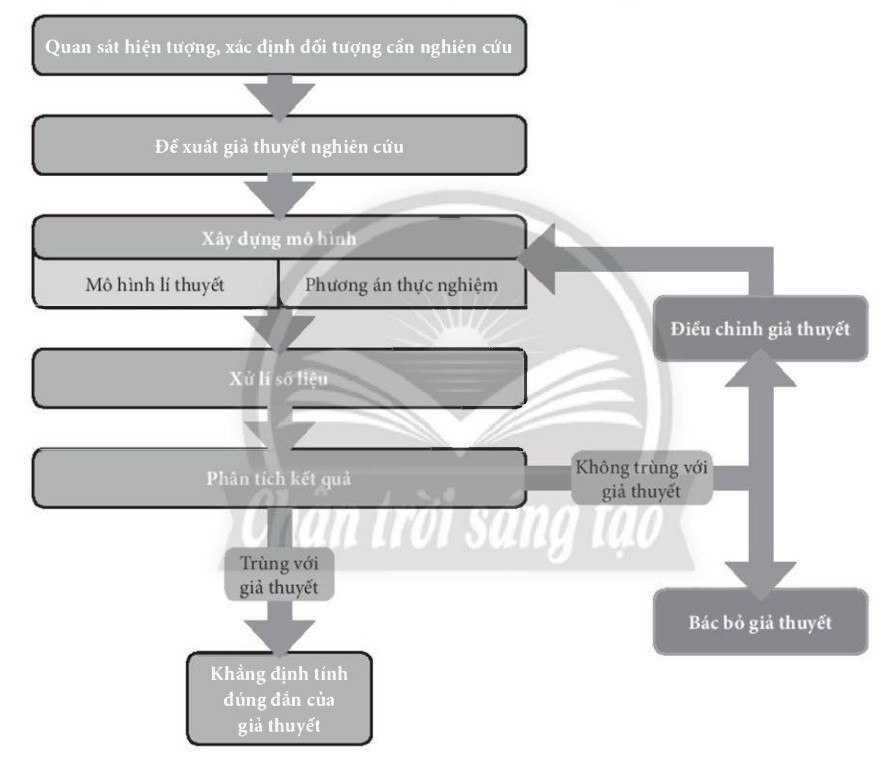
\includegraphics[width=0.9\linewidth]{figs/BAI1-1}
\end{center}